%!TEX root = ../template.tex
%%%%%%%%%%%%%%%%%%%%%%%%%%%%%%%%%%%%%%%%%%%%%%%%%%%%%%%%%%%%%%%%%%%
%% chapter1.tex
%% NOVA thesis document file
%%
%% Chapter with introduciton
%%%%%%%%%%%%%%%%%%%%%%%%%%%%%%%%%%%%%%%%%%%%%%%%%%%%%%%%%%%%%%%%%%%

\typeout{NT LOADING FILE chapter1.tex}

\chapter{Introduction}
\label{cha:introduction}

%% You may define new commands in the main text.  These commands will 
%% be valid from this point until the end of the document.
 

% epigraph configuration
\epigraphfontsize{\small\itshape}
\setlength\epigraphwidth{12.5cm}
\setlength\epigraphrule{0pt}

\epigraph{
  This work is licensed under the \href{LaTeX project public license}{\LaTeX\ Project Public License v1.3c}.
  To view a copy of this license, visit \url{LaTeX project public license}.
}

\section{The \emph{NOVAthesis} template}
\label{sec:a_bit_of_history}

The \gls{novathesis} was initially directed to the PhD and MSc students thesis at \gls{DI} of the \gls{FCT} of the \gls{NOVA}, Portugal, but currently (v5.1.5) it supports other degrees and Schools, namely:
\begin{itemize}
    \newcommand{\mysmallcoversize}{0.09\linewidth}
  \item NOVA University Lisbon
      \begin{itemize}
          \item[]
          \begin{tabularx}{\linewidth}{cX}
              \fbox{
\includegraphics[width=\mysmallcoversize]{cover-phd-nova-fct}} &
              NOVA School of Science and Technology \href{https://www.fct.unl.pt}{(FCT-NOVA)}\\
              \fbox{
\includegraphics[width=\mysmallcoversize]{cover-phd-nova-fcsh}} &
              NOVA School of Social Sciences and Humanities (\href{https://www.fcsh.unl.pt}{FCSH-NOVA})\\
              \fbox{
\includegraphics[width=\mysmallcoversize]{cover-phd-nova-ims}} &
              NOVA Information Management School (\href{https://www.novaims.unl.pt}{NOVA-IMS})\\
              \fbox{
\includegraphics[width=\mysmallcoversize]{cover-phd-nova-ensp}} &
              National School of Public Heath (\href{https://www.ensp.unl.pt}{ENSP-NOVA})\\
          \end{tabularx}
      \end{itemize}
  \item University of Lisbon
      \begin{itemize}
          \item[]
          \begin{tabularx}{\linewidth}{cX}
              \fbox{
\includegraphics[width=\mysmallcoversize]{cover-phd-ul-ist}} &
              Instituto Superior Técnico (\href{https://tecnico.ulisboa.pt}{IST-UL})\\
              \fbox{
\includegraphics[width=\mysmallcoversize]{cover-phd-ul-fc}} &
              Faculdade de Ciências (\href{https://ciencias.ulisboa.pt}{FC-UL})\\
          \end{tabularx}
      \end{itemize}
  \item Instituto Politécnico de Lisboa
      \begin{itemize}  
          \item[]
          \begin{tabularx}{\linewidth}{cX}
              \fbox{
\includegraphics[width=\mysmallcoversize]{cover-phd-ipl-isel}} &
              Instituto Superior de Engenharia de Lisboa (\href{https://www.isel.pt}{ISEL-IPL})\\
          \end{tabularx}
      \end{itemize}
  \item Instituto Politécnico de Setúbal
      \begin{itemize}  
          \item[]
          \begin{tabularx}{\linewidth}{cX}
              \fbox{
\includegraphics[width=\mysmallcoversize]{cover-phd-ips-ests}} &
              Escola Superior de Tecnologia de Setúbal (\href{https://www.estbarreiro.ips.pt}{ESTS-IPS})\\
          \end{tabularx}
      \end{itemize}
  \item Escola Superior de Enfermagem do Porto (\href{https://www.esenf.pt/pt/}{ESEP})
      \begin{itemize}  
          \item[]
          \begin{tabularx}{\linewidth}{cX}
              \fbox{
\includegraphics[width=\mysmallcoversize]{cover-phd-esep}} &
              Escola Superior de Enfermagem do Porto (\href{https://www.esenf.pt/pt/}{ESEP})\\
          \end{tabularx}
      \end{itemize}
\end{itemize}

\section{Getting Started}
\label{sec:getting_started}

The template provides an \emph{easy to use} setting for you to write your thesis/dissertation in \LaTeX:
\begin{itemize}
  \item  Select your school;
  \item Fill your thesis metadata (title, research field, etc) in the file “\texttt{template.tex}”;
  \item Create your thesis/dissertation contents using the files in folder “\texttt{Chapters}”; and
  \item Process using you favorite \LaTeX\ processor (pdf\LaTeX, \XeLaTeX\ or \LuaLaTeX).
\end{itemize}

\subsection{Using Overleaf}
\label{sub:using_overleaf}

\begin{wrapfigure}{r}{0.5\linewidth}
\vspace*{-15ex}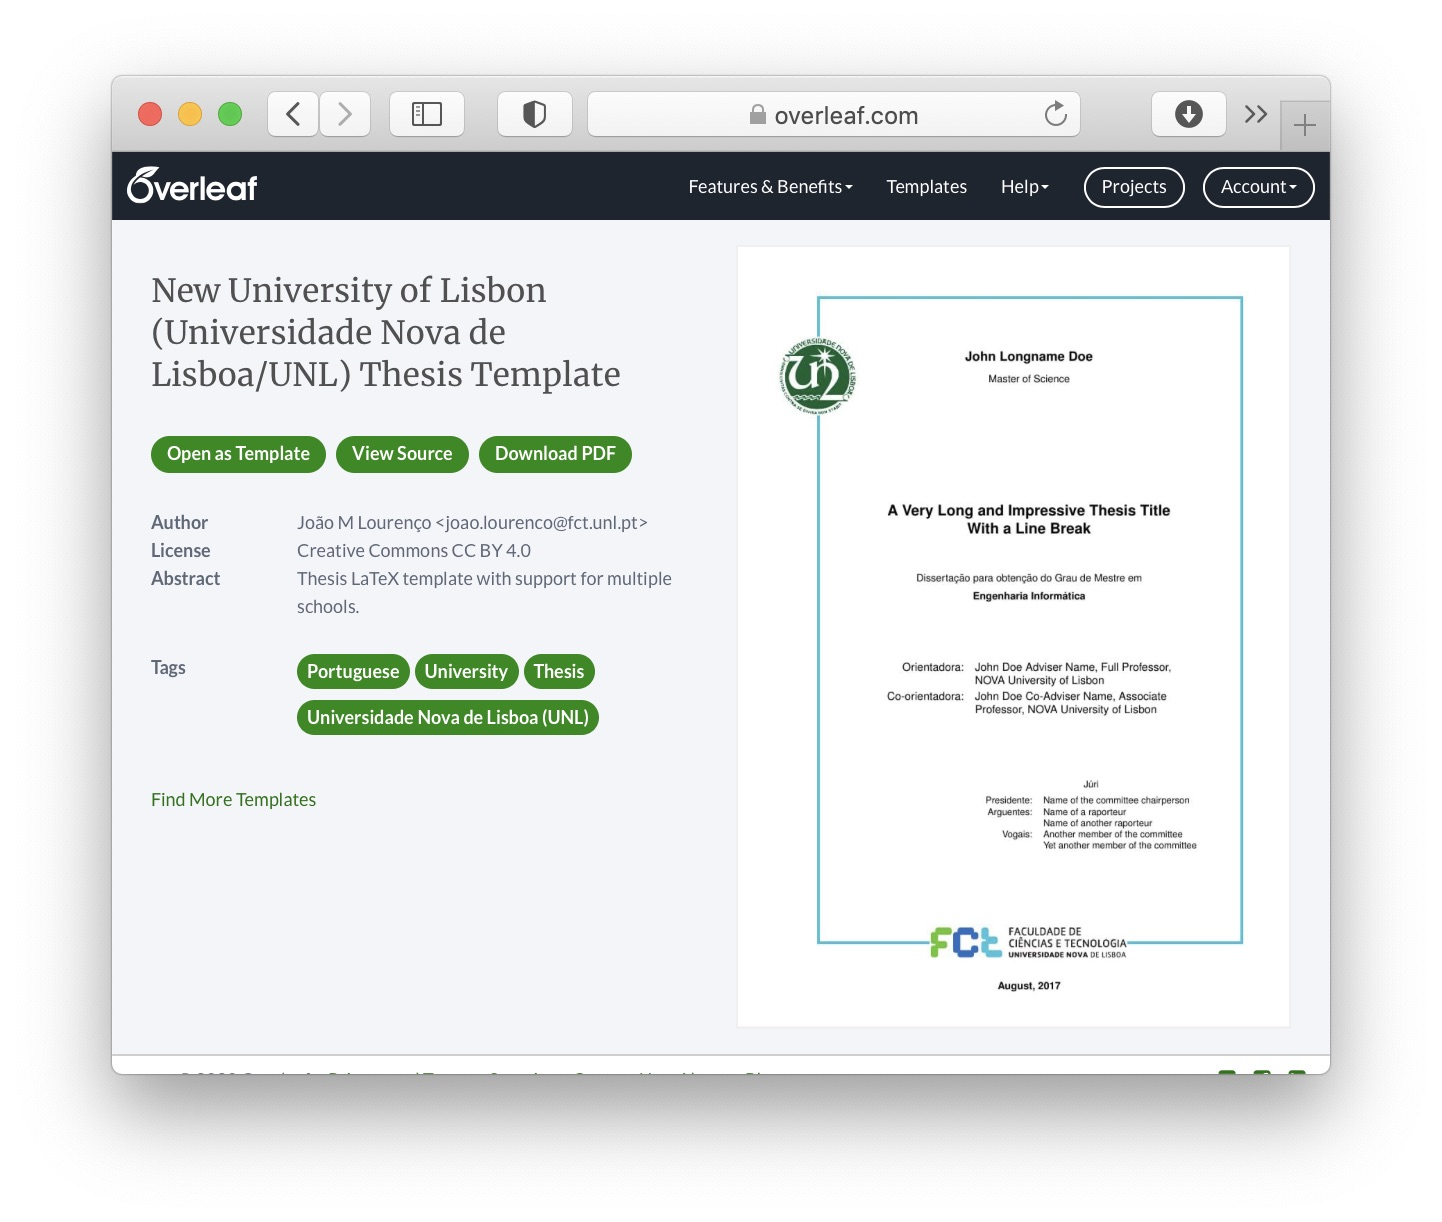
\includegraphics[width=\linewidth]{overleaf}%
\end{wrapfigure}

If you do not have an account in \href{https://www.overleaf.com?r=f5160636&rm=d&rs=b}{Overleaf}, you must \href{https://www.overleaf.com?r=f5160636&rm=d&rs=b}{create one first}.

Onde you have an account, please access the \glsxtrlong{novathesis} in \href{https://www.overleaf.com/latex/templates/new-university-of-lisbon-universidade-nova-de-lisboa-slash-unl-thesis-template/fwbztcrptjmg}{Overleaf} and select the green button \emph{Open as Template}. 

\emph{Please note that the version currently available in Overleaf (v4.1.3) is outdated. A new version will be submitted to Overleaf soon.}  

\subsection{Using a Local \LaTeX\ Installation}
\label{sub:using_local_latex}

\begin{wrapfigure}{r}{0.5\linewidth}
\vspace*{-15ex}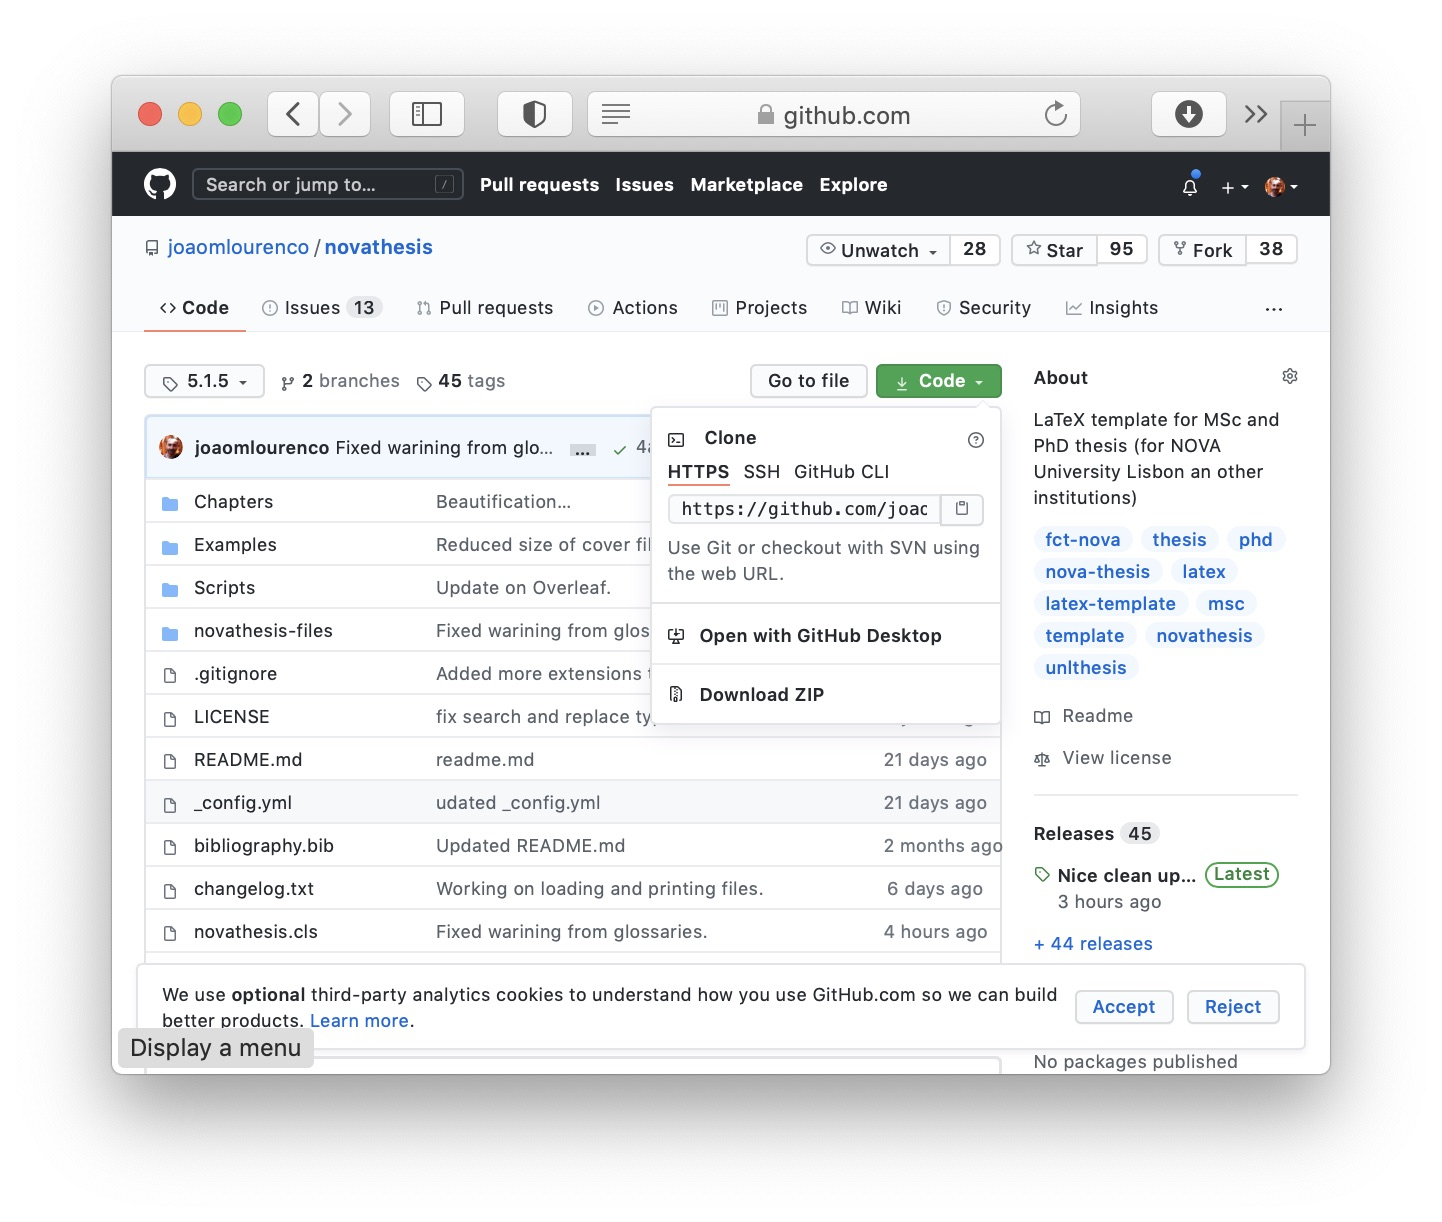
\includegraphics[width=\linewidth]{github}%
\end{wrapfigure}

Just access the \glsxtrlong{novathesis} in \href{https://github.com/joaomlourenco/novathesis}{GitHub}, select the green button \emph{Code} and then \emph{download} (or \emph{clone}) the template.  You will always get the latest version of the template (currently v5.1.8).


\section{Getting Help}
\label{sec:getting_help}

\begin{center}  
  \fbox{\textbf{Please do not send me emails!  I will not answer them!}}
\end{center}
 
\subsection{Google}
\label{sub:group_google}

Remember, when looking for hints or help, \emph{\href{google.com}{Google} is your best friend}!   And if you prefix your Google query with “\emph{LaTeX}”, your fist link will most probably direct you to \texttt{tex.stackexchange.com}.

\subsection{Group Support}
\label{sub:group_support}

To get directed help on the \glsxtrlong{novathesis} please join:
\begin{itemize}
  \item the \href{https://www.facebook.com/groups/novathesis}{NOVAtheis Facebook group}, or
  \item the \href{https://groups.google.com/forum/#!forum/novathesis}{NOVAthesis Google group}.
\end{itemize}

There were huge changes from version 4.x.y to version 5.a.b so, please, \textbf{always} state the version number you are using when asking for help.

\subsection{Reporting Problems}
\label{sub:reporting_problems}

If you just need some help, see above Sections~\autoref{sub:group_google} and~\autoref{sub:group_support}.

If you believe \emph{you found a bug} or if \emph{you need some improvement} in the template, please \href{https://github.com/joaomlourenco/novathesis/issues}{fill an issue in github} at \url{https://github.com/joaomlourenco/novathesis/issues}.


\section{Donations}
\label{sec:donations}

This template is the result of hundreds (yes! \emph{may hundreds}!) of hours of work from the \href{https://docentes.fct.unl.pt/joao-lourenco}{main developer}.  If you think this template really made you life easier while writing your thesis, please consider \href{https://paypal.me/novathesis}{\textbf{making a donation}}. We will keep a list thanking to all the identified donors that identify themselves in the “\emph{Add special instructions to the seller}” box.

\subsubsection*{Donnors 2020}
\label{ssub:donnors_2020}

\begin{inparaitem}[]
  \item João Carvalho, 
  \item David Romão, 
  \item DisplayersereStream, and
  \item António Estêvão.  
\end{inparaitem}

\subsubsection*{Donnors 2019}
\label{ssub:donnors_2019}

\begin{inparaitem}[]
  \item Jorge Barreto and
  \item Raissa Almeida.  
\end{inparaitem}



\section{Disclaimer}
\label{sec:disclaimer}

Although this template is endorsed by the FCT-NOVA and even \href{https://www.fct.unl.pt/estudante/informacao-academica}{linked from its web site}, this is stil not an official template.
%
This template exists to make your life easier and we do our best to make the \gls{novathesis} template compliant to the supported Schools' regulations, but in the end of the line you and only you are accountable for both the look and the contents of the document you submit as your thesis/dissertation.

% \printbibliography[heading=subbibliography, segment=\therefsegment, title={\bibname\ for chapter~\thechapter}]
